\label{sec:arch}
A diagram showing the architecture can be seen in figure \ref{fig:arch} which will be referred to throughout this section.

\begin{figure}[t]
	\centering
	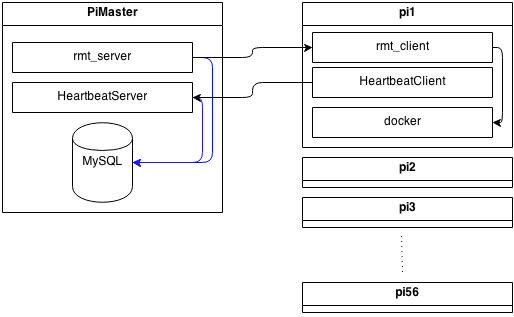
\includegraphics[width=0.6\textwidth]{rmtArch}
	\caption{diagram showing the architecture of \emph{rmt}}
	\label{fig:arch}
\end{figure}

\subsection{Overview}
The PiMaster has the \verb%rmt_server% application running which serves the web pages and retrieves data from the MySQL database and instances of \verb%rmt_client%.
PiMaster also has \verb%HeartbeatServer% running which listens on a specific port for messages from instances of \verb%HeartbeatClient%.

\verb%rmt_server% sends requests to \verb%rmt_client% via a REST interface \citep{rest} for various pieces of information, the details of which are explained further in section \ref{sec:rmt_client}.
Both \verb%rmt_server% and \verb%rmt_client% are web servers, the difference in names is to differentiate the server application from the application meant to be run on the hosts.

All of the Pi hosts have a software stack consisting of \verb%rmt_client%, \verb%HeartbeatClient%, and \verb%docker%.
There is no communication between \verb%rmt_client% and \verb%HeartbeatClient%.
\verb%rmt_client% and \verb%docker% communicate via a python wrapper module discussed in section \ref{impl:dockerpy}.

\subsection{Docker}
The docker module seen in the architecture diagram is docker running on the client.
Docker and its uses are explained in section \ref{sec:docker}.

\subsection{rmt\_client}
\label{sec:rmt_client}
The name of this module is somewhat misleading in that it is not a client at all.
It is actually a \verb%web.py% application and therefore a web server, exposing the following RESTful interface.

\begin{description}
	\item[GET /cpu] returns a \verb%json% object corresponding to the cpu usage of the host as a list of floating point numbers representing percentages of CPU used of the following format: [user, nice, system, idle, iowait, irq, softirq, steal, guest, guest\_nice].
	\item[GET /ram] returns a \verb%json% object corresponding to the ram usage and total ram available in bits.
	\item[GET /temperature] returns a \verb%json% object containing a string with the temperature expressed in millicentigrades.
	\item[GET /containers] returns a \verb%json% object containing the equivalent output to the terminal command, \verb%docker ps%, which lists all currently running containers.
	\item[GET /reboot] returns a \verb%json% object containing a message stating how many seconds it will be before a reboot takes place, and reboots the host.
\end{description}

Given that docker functions must be run as the administrative user, root, on Linux, \verb%rmt_client% itself must be run as root.
This also allows the client to issue the reboot command.

\subsection{MySQL Database}
The database for rmt consists of a single table representing a host named hosts.
This table contains the following fields:

%CREATE TABLE IF NOT EXISTS hosts (
% 	id serial,
% 	address varchar(64),
% 	port int,
% 	tower varchar(8),
% 	last_contacted timestamp,
% 	primary key (id)
%);
\begin{description}
	\item[id] an integer to represent the unique identifier for this host (primary key)
	\item[address] a varchar field to store the hostname or IP address of the host
	\item[port] an integer to store the port of the host
	\item[tower] a varchar to store the tower the host belongs to
	\item[last\_contacted] a timestamp value representing the last time a heartbeat was received from the host
\end{description}

\subsection{HeartbeatServer and HeartbeatClient}
\label{sec:heartbeat}
Both of these are not original to \emph{rmt} as they were retrieved from \url{http://code.activestate.com/recipes/52302-pyheartbeat-detecting-inactive-computers/} and this is stated as such in the comments of the source code.
However they were altered for use in \emph{rmt}.

The HeartbeatServer component is listening on a particular (configurable) port for packets sent by HeartbeatClient.
Once these packets are received, the HeartbeatServer updates the sending host's corresponding last\_contacted field in the hosts table of the database with the current time in a MySQL compatible format.

The number of seconds between each sent packet is configurable on HeartbeatClient, allowing for more or less accuracy depending on requirement.
This number must be a whole number, ie integer.

\subsection{rmt\_server}
\label{sec:rmt_server}

In accordance with the \verb%web.py% framework \citep{webpy}, each web page is assigned a class and that class deals with the logic behind the request either by using the class's \verb%GET% or \verb%POST% method, depending on the type of HTTP request.
The functions not defined as \verb%GET% or \verb%POST% are not exposed via a web interface and are simply regular python functions, following regular python scoping rules.

For example, the \verb%add% class in \verb%rmt_server.py% has three functions: \verb%GET%, \verb%POST%, and \verb%try_host%.
In this example, \verb%try_host% is inaccessible from the web, but is used within the \verb%POST% method to error check the host address being added by the user.

All of the \verb%GET% requests return a rendering of a particular template file.
These template files are HTML (HyperText Markup Language) files representing the web page presented to the user.
Data can be sent to the template as arguments to the render function.
To make this more extensible, \emph{rmt} uses a dictionary object to pass variables to the templates.

For example in the host class's \verb%GET% method, a dictionary is passed to the template with the temperature, RAM usage, CPU usage, among others.
This allows for some entries to be non-existant, or \verb%None% value in python, which means that not all of the information has to be retrieved for the web page to be displayed, giving the application robustness.
In the case that a \verb%None% value is found, such as when a request is made to a host not running \verb%rmt_client%, this is translated in the template to a user-friendly output, as can be seen in the following code sample:

\begin{lstlisting}[caption={Source code snippet from host.html template file}, label={lst:hostWebpy}]
CPU (%)
$if render['cpu_usage'] >= 0:
	<span class="label label-$render['cpu_state']">
		$render['cpu_usage']
	</span>
$else:
	<span class="label label-default">
		Unknown
	</span>
\end{lstlisting}

This shows how the template decides whether to show the left image or right image in figure \ref{fig:cpuGreenUnknown}, using \verb%web.py%'s templating language.
The lines beginning with the dollar sign(\$) (lines 2 and 6) are essentially python, just written within the HTML file.
So in this case, the code displays a Bootstrap label with its colour corresponding to its state (described in section \ref{sec:hbstate}), or if it does not exist, displays a grey (label-default) label with ``Unknown'' within it.

\begin{figure}[t]
	\centering
	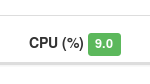
\includegraphics[scale=0.5]{cpuGreen}
	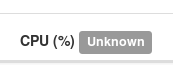
\includegraphics[scale=0.5]{cpuUnknown}
	\caption{Left: CPU data found and displaying value with green label, Right: CPU data unknown with grey label}
	\label{fig:cpuGreenUnknown}
\end{figure}

The values themselves are retrieved from the hosts via \verb%rmt_client%'s RESTful interface described earlier using the \verb%requests% python module.

\subsection{Database Layer}

All database operations are completed through a wrapper, rather than directly via URLs for example.
This adds security to the application as it mitigates the chance of someone performing database actions by accident or intentionally in the case of SQL injection \citep{sqlinjection}.

It also allows for other databases to be used with minimal change to the source code since the database can be initialised using a PostgreSQL \citep{postgresql} database instead of a MySQL one simply by changing the database object constructor and possibly the database creation script, described further in section \ref{sec:future}.
